\documentclass{article}

\usepackage[T1]{fontenc} 
\usepackage[utf8]{inputenc}
\usepackage[francais]{babel}
\usepackage{graphicx}

\title{Rapport Projet Programmation}
\author{Groupe A : Ali Cherifi, Valentin Gaillard, Julien Pilleux}
\date{23/04/2016}

\begin{document}
\maketitle

\newpage

\section {Les objectifs}
\subsection {Objectifs atteints}
Au sein de ce projet, plusieurs objectifs nous ont été fixés et nous avons essayé de tous les remplir.
Les objectifs accomplis sont donc les suivants : \\
\begin{itemize}
\item La version 1 de RushHour a été rendue en temps et en heure et pleinement fonctionnelle. Certains bugs étaient encore présent mais aucun de ses bugs n'étaient pénalisant pour jouer à la première version du jeu.\\

\item La remise de la version 2 s'est elle aussi effectuée sans aucun bug majeur. De plus, les bugs présent dans la première version ont pu être corrigés. Notre code étant fait de manière à être facilement maintenable, nous n'avions que très peu de changement à opérer afin d'inclure le puzzle de l'âne rouge dans le projet. Rendre un code maintenable étant un élément important au sein d'un projet, nous pouvons dire que nous l'avons accompli.\\

\item Un des autres objectifs accompli a été de rendre un code commenté et lisible par autrui. En effet, la relecture croisée nous a permis de nous rendre compte que note code était suffisamment commenté pour permettre une lecture plus aisé au groupe qui nous a évalué. Cela nous a également permis d'apprendre à rédiger des commentaires dans une forme correcte.\\

\item  Un des autres gros objectifs principaux à accomplir a été le solveur. En ayant pensé, écrit et conçu l'algorithme de résolution, nous avons réussi à implémenter un algorithme "naïf" permettant la résolution de jeu simples de RushHour et de l'Ane rouge. Nous avons donc réussi à partir de zéro pour implémenter un solveur fonctionnel.\\

\item Un des autres objectifs accompli a été l'apprentissage et l'utilisation d'une librairie externe ç celles proposées de base par C, la SDL. Nous avons pu créer une interface graphique simple mais fonctionelle pour notre jeu nous montrant notre progression depuis le début du projet.\\

\item Au travers de ce projet nous avons également développé nos compétences dans l'utilisation des ressources et outils offert en programmation. Nous sommes désormais capables d'utiliser les outils de débuggage en terminal ou dans un IDE, de nous servir des programmes de gestion de contrôle de version (GIT/SVN), et des programmes de contrôle de la mémoire (valgrind).\newpage
\end{itemize}

\subsection {Objectifs non atteints}
\begin{itemize}
\item Tout d'abord, nous avons les nombreuses fuites mémoires contenues dans le solveur. Celles ci sont importantes et nous ne sommes pas parvenues à les éliminer malgré nos recherches et l'aide des outils proposés.\\

\item Ensuite, nous avons le fait que le solveur ne peut pas résoudre des jeux trop compliqués. Le solveur sature vite, fait beaucoup trop d'allocation mémoire, et met énormément de temps à résoudre des jeux complexes. Il nous a également été possible de voir grâce à la compétition de solveur qu'il ne retournait pas forcément une valeur correcte. Il faudrait donc revoir son implémentation ainsi que peut être celle du tas et de la file.\\

\item Dans les objectifs non accomplis nous avons également la non documentation via Doxygen. Cela peut devenir très embêtant si nous avions dû donner une librairie contenant par exemple la pile et le tas. Le programmeur en utilisant cette librairie n'aurait eu aucun moyen de connaître les services offerts par cette librairie dans disposer des fichiers d'en-tête. Nous ne sommes donc pas en mesure de fournir une librairie complète.   
\end{itemize}

\section {Problème technique}
\subsection {L'affichage dans le terminal}
Au moment d'afficher notre jeu dans le terminal, nous avons cherché à avoir une grille et des instructions les plus propres possibles. Nous avons déjà eu recours au printf classique, mais l'affichage se faisais en dessous et s'empilait ainsi dans le terminal. Cela ne nous convenait pas alors nous avons entendu parlé d'une méthode nous permettant de ré-afficher par dessus ce que nous avons déjà inscrit. Il fallait toujours utiliser printf mais avec des paramètres supplémentaires au début de celle-ci.
\subsection {Les paramètres de la fonction printf}

\begin{flushleft}

\includegraphics[scale=0.45]{printf_capture.png}
\end{flushleft}

Ce paramètre additionnel nous a permis de pouvoir choisir, directement dans le terminal, où écrire. Le premier paramètre entier, nous permet de choisir quelle est la ligne du terminal nous allons écrire, la ligne est choisie à partir de la vu courante, elle est donc comptée depuis la première ligne affichée du terminal. Ici la variable instruction line correspond à la ligne en dessous de la grille. Un autre problème rencontré est que à chaque affichage de la grille, la vue courante du terminal changeait, donc pour avoir toujours la même ligne à chaque tour de boucle, il a juste fallut ajouter une fonction permettant de clean l'affichage du terminal (System (``clear'')).
Le second paramètre entier correspond tout simplement au nombre de caractère qu'il faut laisser entre le bord gauche du terminal et le premier caractère de la chaîne de caractère que l'on veut afficher. Ici, le fait de mettre 0 permet de coller la chaîne au bord du terminal.
Finalement, le dernier paramètre, la chaîne de caractère est tout simplement la chaîne à afficher aux coordonnées précédemment choisies. Avec ceci, nous obtenons un affichage propre.

\subsection {Le retour à la ligne du prompt}
Même avec ce printf, il nous restait le soucis du prompt qui revenait à la ligne, et les options saisies ne s'affichait pas sur la même ligne. En effet, une fois une option saisie, le curseur se positionnait automatiquement sur la ligne d'en dessous. Pour palier à ça, il a fallut créer une fonction reset cursor qui replaçait le prompt sur la bonne ligne.

\begin{flushleft}
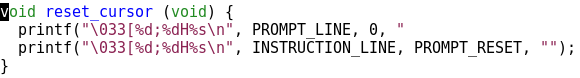
\includegraphics[scale=0.45]{reset_cursor.png}
\end{flushleft}

Cette fonction utilise le printf précédemment vu. Le premier printf sert à réinitialiser la ligne de saisie afin qu'elle apparaisse vide, pour que la prochaine saisie puisse être entrée sans chevauchement de caractères. Puis, la seconde instruction nous sert à imprimer une chaîne de caractère vide sur la ligne au dessus de la ligne de la saisie, pour que le curseur se positionne automatiquement sur cette dernière.

\section {Redondance de code}
Valentin

\end{document}
